\documentclass[11pt]{article}
\usepackage{mathblatt}
% gesetzt von werkzeuge/setzer.py (Sorte selbst) aus dem Lernweg 6KD
% und den Bankzeilen; Muster bau/proben/2026-10-09/hypotenuse-muster.
\usepackage{enumitem}
\usepackage{adjustbox,varwidth}
\newgeometry{a4paper,margin=18mm,top=15mm,bottom=20mm,footskip=9mm}
\pagestyle{fancy}\fancyhf{}\renewcommand{\headrulewidth}{0pt}
\fancyfoot[L]{\footnotesize\color{mbgrau}6KD \textperiodcentered{} Baumdiagramm und Pfadregeln}
\fancyfoot[R]{\footnotesize\color{mbgrau}\thepage}
\setlength{\parskip}{3pt}
\renewcommand{\kreuz}[1]{\mbox{$\square$\ #1}\quad}
\newcommand{\kreuzl}[1]{\par\hangindent1.4em\hangafter1\noindent$\square$\ #1}
\newcommand{\aufg}[3]{\par\noindent\makebox[0pt][r]{#3}\begin{minipage}[t]{\linewidth}#1\end{minipage}\par}
\newcommand{\aufgg}[4]{\par\noindent\makebox[0pt][r]{#4}\begin{minipage}[t]{0.6\linewidth}\vspace{0pt}#1\end{minipage}\hfill
  \begin{minipage}[t]{0.37\linewidth}\vspace{0pt}\centering #2\end{minipage}\par}
\newcommand{\nr}[1]{\makebox[7mm][l]{\textbf{#1}}}
\newcommand{\lsg}[3]{\par\noindent\begin{minipage}[t]{9mm}\textbf{#1}\end{minipage}%
  \begin{minipage}[t]{52mm}\raggedright\bfseries\boldmath #2\end{minipage}\hspace{3mm}%
  \begin{minipage}[t]{\dimexpr\linewidth-64mm\relax}\raggedright\small #3\end{minipage}\par\vspace{4pt}}
\newlength{\kr}
\makeatletter
\newcommand{\karomerk}[2]{\protected@write\@auxout{}{\string\karoseite{#1}{#2}{\thepage}}}
\newcommand{\karoseite}[3]{\expandafter\xdef\csname karo@#1@#2\endcsname{#3}}
\newcommand{\karohinweis}[3]{\karomerk{h}{#1}\ifcsname karo@k@#1\endcsname
  \ifnum\csname karo@k@#1\endcsname=0\csname karo@h@#1\endcsname\relax#2\else#3\fi
  \else#3\fi}
\makeatother
\begin{document}

\noindent{\LARGE\bfseries Baumdiagramm und Pfadregeln}\par\smallskip
\noindent{\small\color{mbgrau}Selbstlernheft Klasse 9 \textperiodcentered{} mit Lösungsheft \textperiodcentered{} Kennung 6KD}\par\medskip
\noindent\textbf{So nutzt du das Heft:} Lies im Abschnitt das Beispiel. Rechne dann die Aufgaben der Reihe nach und vergleiche jede sofort mit dem Lösungsheft. Kreuze „kann ich“ an, wenn du die letzte Aufgabe (\emph{Ziel}) allein schaffst.\par
\noindent Mehr Aufgaben zu einem Abschnitt: Kennung deinem Nachhilfelehrer schicken (z.\,B. „6KD mehr B“).\par\medskip
{\arrayrulecolor{mbgrau}\renewcommand{\arraystretch}{1.3}
\noindent\begin{tabular}{|>{\bfseries}p{10mm}|p{112mm}|>{\raggedleft\arraybackslash}p{10mm}|>{\centering\arraybackslash}p{14mm}|}\hline
\rowcolor{black!8} & \textbf{Abschnitt} & \textbf{Seite} & \textbf{kann ich}\\\hline
A & Baum und Pfadregel & \pageref{s:A} & $\square$\\\hline
B & Mehrere Pfade: plus & \pageref{s:B} & $\square$\\\hline
C & Mindestens einmal: über das Gegenteil & \pageref{s:C} & $\square$\\\hline
D & Drei Stufen & \pageref{s:D} & $\square$\\\hline
T & Probetest & \pageref{s:T} & $\square$\\\hline
\end{tabular}}\par\bigskip

\begin{tcolorbox}[colback=mbkasten,colframe=mbgrau,boxrule=0.5pt,arc=1mm,left=3mm,right=3mm,top=2mm,bottom=2mm,title={\bfseries Formel auf einen Blick},coltitle=black,colbacktitle=black!10]
{\Large Pfad: mal \qquad mehrere Pfade: plus \\ mindestens einmal: Gegenteil rechnen, von 1 abziehen}\par\medskip
\textbf{So gehst du vor}\par
\nr{1}Baum zeichnen, an jeden Ast seine Wahrscheinlichkeit\par
\nr{2}die Pfade suchen, die zum Ereignis gehören\par
\nr{3}je Pfad multiplizieren\par
\nr{4}die Pfade addieren\par
\medskip
\end{tcolorbox}
\clearpage\label{s:A}\noindent\colorbox{black!12}{\makebox[10mm]{\Large\bfseries\strut A}}\hspace{3mm}{\Large\bfseries Baum und Pfadregel}\par\smallskip
\noindent Im Baum steht an jedem Ast die Wahrscheinlichkeit für diese Stufe; die Äste an einem Punkt ergeben zusammen 1. Für ein Ergebnis fährst du seinen Pfad nach und multiplizierst die Äste.\par\medskip
\noindent\textbf{Formel}\par\nopagebreak\noindent\hspace*{4mm}\begin{minipage}{\dimexpr\linewidth-4mm\relax}$P(\text{Pfad}) = P(\text{1. Ast}) \cdot P(\text{2. Ast})$\end{minipage}\par\medskip
\noindent\textbf{Beispiel}\quad Ein Glücksrad hat 4 gleich große Felder: 1 rotes (R) und 3 blaue (B). Es wird zweimal gedreht. Wie groß ist die Wahrscheinlichkeit für zweimal Rot?\par\smallskip
\noindent\begin{minipage}[t]{0.6\linewidth}\vspace{0pt}\par\noindent\hangindent6mm\hangafter1\makebox[6mm][l]{\textbf{1}}1. Stufe: R $\frac{1}{4}$, B $\frac{3}{4}$ – zusammen 1.\par\smallskip\par\noindent\hangindent6mm\hangafter1\makebox[6mm][l]{\textbf{2}}2. Stufe: Das Rad ist dasselbe, also an jedem Punkt wieder $\frac{1}{4}$ und $\frac{3}{4}$.\par\smallskip\par\noindent\hangindent6mm\hangafter1\makebox[6mm][l]{\textbf{3}}Pfad R – R nachfahren und multiplizieren: $\frac{1}{4} \cdot \frac{1}{4} = \frac{1}{16}$.\par\smallskip\par\noindent\hangindent6mm\hangafter1\makebox[6mm][l]{\textbf{4}}Die Wahrscheinlichkeit für zweimal Rot ist $\frac{1}{16}$.\par\smallskip\end{minipage}\hfill
\begin{minipage}[t]{0.37\linewidth}\vspace{0pt}\centering 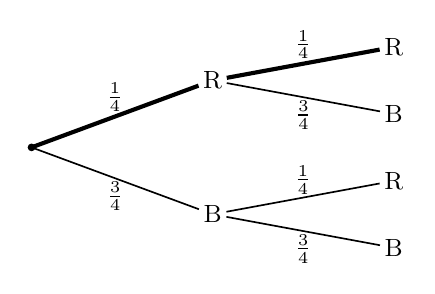
\begin{tikzpicture}[ak/.style={font=\small,inner sep=1.5pt,fill=white},wk/.style={font=\footnotesize,inner sep=1pt}]\fill (0,0) circle (1.4pt);\coordinate (s) at (0,0);\node[ak] (n0) at (2.30,0.850) {R};\node[ak] (n1) at (2.30,-0.850) {B};\node[ak] (n00) at (4.60,1.275) {R};\node[ak] (n01) at (4.60,0.425) {B};\node[ak] (n10) at (4.60,-0.425) {R};\node[ak] (n11) at (4.60,-1.275) {B};\draw[line width=1.5pt] (s) -- (n0) node[wk,above,pos=0.5] {$\frac{1}{4}$};\draw[line width=0.6pt] (s) -- (n1) node[wk,below,pos=0.5] {$\frac{3}{4}$};\draw[line width=1.5pt] (n0) -- (n00) node[wk,above,pos=0.5] {$\frac{1}{4}$};\draw[line width=0.6pt] (n0) -- (n01) node[wk,below,pos=0.5] {$\frac{3}{4}$};\draw[line width=0.6pt] (n1) -- (n10) node[wk,above,pos=0.5] {$\frac{1}{4}$};\draw[line width=0.6pt] (n1) -- (n11) node[wk,below,pos=0.5] {$\frac{3}{4}$};\end{tikzpicture}\end{minipage}\par\medskip
\noindent\textbf{Aufgaben}\hspace{1em}{\small\color{mbgrau}\karohinweis{A}{Rechne unten im Karo.}{Rechne auf einem extra Blatt.} Vergleiche jede Aufgabe gleich mit dem Lösungsheft.}\par\smallskip
\aufgg{\hangindent7mm\hangafter1\nr{1.}Eine Münze wird zweimal geworfen (K Kopf, Z Zahl). Trage im Baum an jeden Ast die Wahrscheinlichkeit ein. Wie groß ist die Wahrscheinlichkeit für zweimal Zahl?}{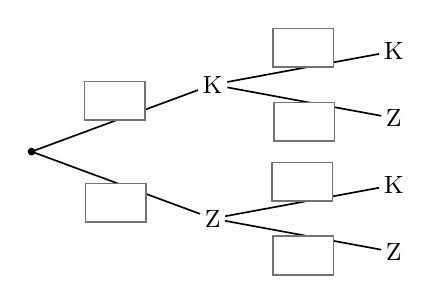
\begin{tikzpicture}[ak/.style={font=\small,inner sep=1.5pt,fill=white},wk/.style={font=\footnotesize,inner sep=1pt}]\fill (0,0) circle (1.4pt);\coordinate (s) at (0,0);\node[ak] (n0) at (2.30,0.850) {K};\node[ak] (n1) at (2.30,-0.850) {Z};\node[ak] (n00) at (4.60,1.275) {K};\node[ak] (n01) at (4.60,0.425) {Z};\node[ak] (n10) at (4.60,-0.425) {K};\node[ak] (n11) at (4.60,-1.275) {Z};\draw[line width=0.6pt] (s) -- (n0) node[wk,above,draw=black!55,fill=white,pos=0.5] {\rule{0pt}{4.2mm}\rule{7mm}{0pt}};\draw[line width=0.6pt] (s) -- (n1) node[wk,below,draw=black!55,fill=white,pos=0.5] {\rule{0pt}{4.2mm}\rule{7mm}{0pt}};\draw[line width=0.6pt] (n0) -- (n00) node[wk,above,draw=black!55,fill=white,pos=0.5] {\rule{0pt}{4.2mm}\rule{7mm}{0pt}};\draw[line width=0.6pt] (n0) -- (n01) node[wk,below,draw=black!55,fill=white,pos=0.5] {\rule{0pt}{4.2mm}\rule{7mm}{0pt}};\draw[line width=0.6pt] (n1) -- (n10) node[wk,above,draw=black!55,fill=white,pos=0.5] {\rule{0pt}{4.2mm}\rule{7mm}{0pt}};\draw[line width=0.6pt] (n1) -- (n11) node[wk,below,draw=black!55,fill=white,pos=0.5] {\rule{0pt}{4.2mm}\rule{7mm}{0pt}};\end{tikzpicture}}{}{}
\medskip
\aufgg{\hangindent7mm\hangafter1\nr{2.}Ein Glücksrad hat 5 gleich große Felder: 2 gelbe und 3 grüne. Es wird zweimal gedreht. Im Baum steht nur eine Wahrscheinlichkeit. Ergänze die anderen. Wie groß ist die Wahrscheinlichkeit für zuerst Gelb, dann Grün?}{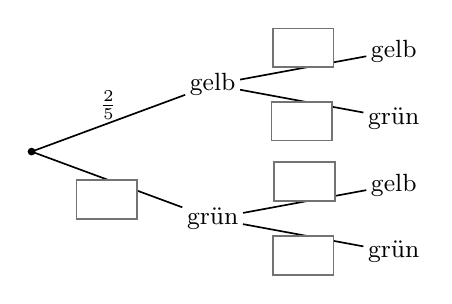
\begin{tikzpicture}[ak/.style={font=\small,inner sep=1.5pt,fill=white},wk/.style={font=\footnotesize,inner sep=1pt}]\fill (0,0) circle (1.4pt);\coordinate (s) at (0,0);\node[ak] (n0) at (2.30,0.850) {gelb};\node[ak] (n1) at (2.30,-0.850) {grün};\node[ak] (n00) at (4.60,1.275) {gelb};\node[ak] (n01) at (4.60,0.425) {grün};\node[ak] (n10) at (4.60,-0.425) {gelb};\node[ak] (n11) at (4.60,-1.275) {grün};\draw[line width=0.6pt] (s) -- (n0) node[wk,above,pos=0.5] {$\frac{2}{5}$};\draw[line width=0.6pt] (s) -- (n1) node[wk,below,draw=black!55,fill=white,pos=0.5] {\rule{0pt}{4.2mm}\rule{7mm}{0pt}};\draw[line width=0.6pt] (n0) -- (n00) node[wk,above,draw=black!55,fill=white,pos=0.5] {\rule{0pt}{4.2mm}\rule{7mm}{0pt}};\draw[line width=0.6pt] (n0) -- (n01) node[wk,below,draw=black!55,fill=white,pos=0.5] {\rule{0pt}{4.2mm}\rule{7mm}{0pt}};\draw[line width=0.6pt] (n1) -- (n10) node[wk,above,draw=black!55,fill=white,pos=0.5] {\rule{0pt}{4.2mm}\rule{7mm}{0pt}};\draw[line width=0.6pt] (n1) -- (n11) node[wk,below,draw=black!55,fill=white,pos=0.5] {\rule{0pt}{4.2mm}\rule{7mm}{0pt}};\end{tikzpicture}}{}{}
\medskip
\aufgg{\hangindent7mm\hangafter1\nr{3.}Zwei Glücksräder haben je 4 gleich große Felder (Bild). Erst wird das linke, dann das rechte gedreht. Wie groß ist die Wahrscheinlichkeit für zweimal A?}{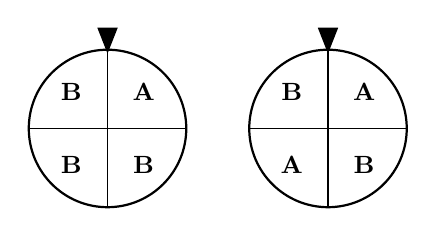
\begin{tikzpicture}[font=\small]\draw[line width=0.5pt] (0.0,0) -- ++(90.00:1.0);\node at ([shift=(45.00:0.65)]0.0,0) {\textbf{A}};\draw[line width=0.5pt] (0.0,0) -- ++(0.00:1.0);\node at ([shift=(-45.00:0.65)]0.0,0) {\textbf{B}};\draw[line width=0.5pt] (0.0,0) -- ++(-90.00:1.0);\node at ([shift=(-135.00:0.65)]0.0,0) {\textbf{B}};\draw[line width=0.5pt] (0.0,0) -- ++(-180.00:1.0);\node at ([shift=(-225.00:0.65)]0.0,0) {\textbf{B}};\draw[line width=0.8pt] (0.0,0) circle (1.0);\fill (0.0,0.95) -- ++(-0.13,0.33) -- ++(0.26,0) -- cycle;\draw[line width=0.5pt] (2.8,0) -- ++(90.00:1.0);\node at ([shift=(45.00:0.65)]2.8,0) {\textbf{A}};\draw[line width=0.5pt] (2.8,0) -- ++(0.00:1.0);\node at ([shift=(-45.00:0.65)]2.8,0) {\textbf{B}};\draw[line width=0.5pt] (2.8,0) -- ++(-90.00:1.0);\node at ([shift=(-135.00:0.65)]2.8,0) {\textbf{A}};\draw[line width=0.5pt] (2.8,0) -- ++(-180.00:1.0);\node at ([shift=(-225.00:0.65)]2.8,0) {\textbf{B}};\draw[line width=0.8pt] (2.8,0) circle (1.0);\fill (2.8,0.95) -- ++(-0.13,0.33) -- ++(0.26,0) -- cycle;\end{tikzpicture}}{}{}
\medskip
\aufgg{\hangindent7mm\hangafter1\nr{4.}Zwei Glücksräder haben je 4 gleich große Felder, noch ohne Buchstaben (Bild). Erst wird das linke, dann das rechte gedreht. Schreibe in jedes Feld A oder B, sodass „zweimal A“ die Wahrscheinlichkeit $\frac{3}{16}$ hat. Zeige es mit einer Rechnung.}{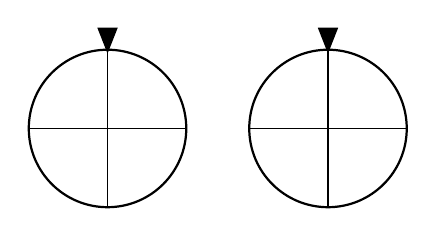
\begin{tikzpicture}[font=\small]\draw[line width=0.5pt] (0.0,0) -- ++(90.00:1.0);\draw[line width=0.5pt] (0.0,0) -- ++(0.00:1.0);\draw[line width=0.5pt] (0.0,0) -- ++(-90.00:1.0);\draw[line width=0.5pt] (0.0,0) -- ++(-180.00:1.0);\draw[line width=0.8pt] (0.0,0) circle (1.0);\fill (0.0,0.95) -- ++(-0.13,0.33) -- ++(0.26,0) -- cycle;\draw[line width=0.5pt] (2.8,0) -- ++(90.00:1.0);\draw[line width=0.5pt] (2.8,0) -- ++(0.00:1.0);\draw[line width=0.5pt] (2.8,0) -- ++(-90.00:1.0);\draw[line width=0.5pt] (2.8,0) -- ++(-180.00:1.0);\draw[line width=0.8pt] (2.8,0) circle (1.0);\fill (2.8,0.95) -- ++(-0.13,0.33) -- ++(0.26,0) -- cycle;\end{tikzpicture}}{}{{\scriptsize\color{mbgrau}Ziel\hspace{2mm}}}
\medskip
\par\vspace{3mm}\setlength{\kr}{\dimexpr\pagegoal-\pagetotal-10mm\relax}%
\ifdim\kr>12mm\karomerk{k}{A}\noindent{\scriptsize\color{mbgrau}Platz zum Rechnen}\par\nointerlineskip\vspace{1mm}\noindent
\begin{tikzpicture}\clip (0,0) rectangle ({\linewidth-0.5mm},\kr);\draw[black!16,line width=0.3pt,step=5mm] (0,0) grid (\linewidth,\kr);\end{tikzpicture}\fi\par
\clearpage\label{s:B}\noindent\colorbox{black!12}{\makebox[10mm]{\Large\bfseries\strut B}}\hspace{3mm}{\Large\bfseries Mehrere Pfade: plus}\par\smallskip
\noindent Gehören mehrere Pfade zum Ereignis, rechnest du jeden Pfad für sich und addierst dann.\par\medskip
\noindent\textbf{Formel}\par\nopagebreak\noindent\hspace*{4mm}\begin{minipage}{\dimexpr\linewidth-4mm\relax}$P(\text{Ereignis}) = P(\text{Pfad 1}) + P(\text{Pfad 2}) + \ldots$\end{minipage}\par\medskip
\noindent\textbf{Beispiel}\quad Ein Glücksrad hat 4 gleich große Felder: 1 rotes (R) und 3 blaue (B). Es wird zweimal gedreht. Wie groß ist die Wahrscheinlichkeit für genau einmal Rot?\par\smallskip
\noindent\begin{minipage}[t]{0.6\linewidth}\vspace{0pt}\par\noindent\hangindent6mm\hangafter1\makebox[6mm][l]{\textbf{1}}Genau einmal Rot: zwei Pfade, R – B und B – R.\par\smallskip\par\noindent\hangindent6mm\hangafter1\makebox[6mm][l]{\textbf{2}}R – B: $\frac{1}{4} \cdot \frac{3}{4} = \frac{3}{16}$; \quad B – R: $\frac{3}{4} \cdot \frac{1}{4} = \frac{3}{16}$.\par\smallskip\par\noindent\hangindent6mm\hangafter1\makebox[6mm][l]{\textbf{3}}Addieren: $\frac{3}{16} + \frac{3}{16} = \frac{6}{16} = \frac{3}{8}$.\par\smallskip\par\noindent\hangindent6mm\hangafter1\makebox[6mm][l]{\textbf{4}}Die Wahrscheinlichkeit für genau einmal Rot ist $\frac{3}{8}$.\par\smallskip\end{minipage}\hfill
\begin{minipage}[t]{0.37\linewidth}\vspace{0pt}\centering 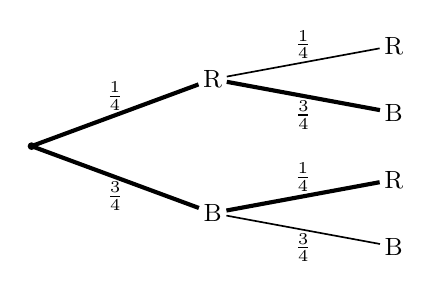
\begin{tikzpicture}[ak/.style={font=\small,inner sep=1.5pt,fill=white},wk/.style={font=\footnotesize,inner sep=1pt}]\fill (0,0) circle (1.4pt);\coordinate (s) at (0,0);\node[ak] (n0) at (2.30,0.850) {R};\node[ak] (n1) at (2.30,-0.850) {B};\node[ak] (n00) at (4.60,1.275) {R};\node[ak] (n01) at (4.60,0.425) {B};\node[ak] (n10) at (4.60,-0.425) {R};\node[ak] (n11) at (4.60,-1.275) {B};\draw[line width=1.5pt] (s) -- (n0) node[wk,above,pos=0.5] {$\frac{1}{4}$};\draw[line width=1.5pt] (s) -- (n1) node[wk,below,pos=0.5] {$\frac{3}{4}$};\draw[line width=0.6pt] (n0) -- (n00) node[wk,above,pos=0.5] {$\frac{1}{4}$};\draw[line width=1.5pt] (n0) -- (n01) node[wk,below,pos=0.5] {$\frac{3}{4}$};\draw[line width=1.5pt] (n1) -- (n10) node[wk,above,pos=0.5] {$\frac{1}{4}$};\draw[line width=0.6pt] (n1) -- (n11) node[wk,below,pos=0.5] {$\frac{3}{4}$};\end{tikzpicture}\end{minipage}\par\medskip
\noindent\textbf{Aufgaben}\hspace{1em}{\small\color{mbgrau}\karohinweis{B}{Rechne unten im Karo.}{Rechne auf einem extra Blatt.} Vergleiche jede Aufgabe gleich mit dem Lösungsheft.}\par\smallskip
\aufgg{\hangindent7mm\hangafter1\nr{1.}Ole wirft zweimal auf den Korb. Der Baum zeigt, wie wahrscheinlich er trifft (T Treffer, D daneben). Wie groß ist die Wahrscheinlichkeit, dass er genau einmal trifft?}{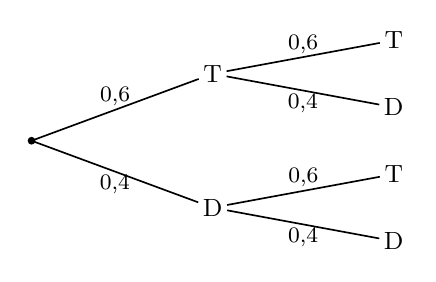
\begin{tikzpicture}[ak/.style={font=\small,inner sep=1.5pt,fill=white},wk/.style={font=\footnotesize,inner sep=1pt}]\fill (0,0) circle (1.4pt);\coordinate (s) at (0,0);\node[ak] (n0) at (2.30,0.850) {T};\node[ak] (n1) at (2.30,-0.850) {D};\node[ak] (n00) at (4.60,1.275) {T};\node[ak] (n01) at (4.60,0.425) {D};\node[ak] (n10) at (4.60,-0.425) {T};\node[ak] (n11) at (4.60,-1.275) {D};\draw[line width=0.6pt] (s) -- (n0) node[wk,above,pos=0.5] {$0{,}6$};\draw[line width=0.6pt] (s) -- (n1) node[wk,below,pos=0.5] {$0{,}4$};\draw[line width=0.6pt] (n0) -- (n00) node[wk,above,pos=0.5] {$0{,}6$};\draw[line width=0.6pt] (n0) -- (n01) node[wk,below,pos=0.5] {$0{,}4$};\draw[line width=0.6pt] (n1) -- (n10) node[wk,above,pos=0.5] {$0{,}6$};\draw[line width=0.6pt] (n1) -- (n11) node[wk,below,pos=0.5] {$0{,}4$};\end{tikzpicture}}{}{}
\medskip
\aufgg{\hangindent7mm\hangafter1\nr{2.}Zwei Glücksräder haben je 4 gleich große Felder (Bild). Erst wird das linke, dann das rechte gedreht. Die beiden Ziffern ergeben eine Zahl. Wie groß ist die Wahrscheinlichkeit für 34 oder 43?}{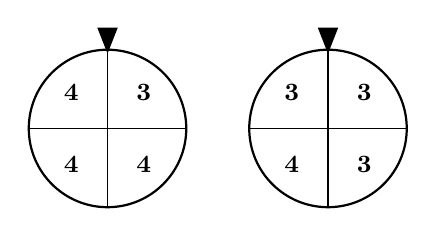
\begin{tikzpicture}[font=\small]\draw[line width=0.5pt] (0.0,0) -- ++(90.00:1.0);\node at ([shift=(45.00:0.65)]0.0,0) {\textbf{3}};\draw[line width=0.5pt] (0.0,0) -- ++(0.00:1.0);\node at ([shift=(-45.00:0.65)]0.0,0) {\textbf{4}};\draw[line width=0.5pt] (0.0,0) -- ++(-90.00:1.0);\node at ([shift=(-135.00:0.65)]0.0,0) {\textbf{4}};\draw[line width=0.5pt] (0.0,0) -- ++(-180.00:1.0);\node at ([shift=(-225.00:0.65)]0.0,0) {\textbf{4}};\draw[line width=0.8pt] (0.0,0) circle (1.0);\fill (0.0,0.95) -- ++(-0.13,0.33) -- ++(0.26,0) -- cycle;\draw[line width=0.5pt] (2.8,0) -- ++(90.00:1.0);\node at ([shift=(45.00:0.65)]2.8,0) {\textbf{3}};\draw[line width=0.5pt] (2.8,0) -- ++(0.00:1.0);\node at ([shift=(-45.00:0.65)]2.8,0) {\textbf{3}};\draw[line width=0.5pt] (2.8,0) -- ++(-90.00:1.0);\node at ([shift=(-135.00:0.65)]2.8,0) {\textbf{4}};\draw[line width=0.5pt] (2.8,0) -- ++(-180.00:1.0);\node at ([shift=(-225.00:0.65)]2.8,0) {\textbf{3}};\draw[line width=0.8pt] (2.8,0) circle (1.0);\fill (2.8,0.95) -- ++(-0.13,0.33) -- ++(0.26,0) -- cycle;\end{tikzpicture}}{}{}
\medskip
\aufg{\hangindent7mm\hangafter1\nr{3.}In einem Beutel liegen 2 rote, 3 blaue und 5 gelbe Kugeln. Es wird zweimal mit Zurücklegen gezogen; dein Baum hat an jedem Punkt drei Äste (rot, blau, gelb). Wie groß ist die Wahrscheinlichkeit für zweimal dieselbe Farbe?}{}{}
\medskip
\aufgg{\hangindent7mm\hangafter1\nr{4.}Mia und Tom spielen mit dem Glücksrad im Bild (6 gleich große Felder). Es wird zweimal gedreht. Kommt zweimal dieselbe Farbe, gewinnt Mia, sonst Tom. Ist das Spiel fair? Begründe mit den Wahrscheinlichkeiten.}{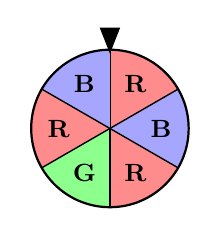
\begin{tikzpicture}[font=\small]\fill[red!45] (0.0,0) -- ++(90.00:1.0) arc (90.00:30.00:1.0) -- cycle;\draw[line width=0.5pt] (0.0,0) -- ++(90.00:1.0);\node at ([shift=(60.00:0.65)]0.0,0) {\textbf{R}};\fill[blue!35] (0.0,0) -- ++(30.00:1.0) arc (30.00:-30.00:1.0) -- cycle;\draw[line width=0.5pt] (0.0,0) -- ++(30.00:1.0);\node at ([shift=(0.00:0.65)]0.0,0) {\textbf{B}};\fill[red!45] (0.0,0) -- ++(-30.00:1.0) arc (-30.00:-90.00:1.0) -- cycle;\draw[line width=0.5pt] (0.0,0) -- ++(-30.00:1.0);\node at ([shift=(-60.00:0.65)]0.0,0) {\textbf{R}};\fill[green!45] (0.0,0) -- ++(-90.00:1.0) arc (-90.00:-150.00:1.0) -- cycle;\draw[line width=0.5pt] (0.0,0) -- ++(-90.00:1.0);\node at ([shift=(-120.00:0.65)]0.0,0) {\textbf{G}};\fill[red!45] (0.0,0) -- ++(-150.00:1.0) arc (-150.00:-210.00:1.0) -- cycle;\draw[line width=0.5pt] (0.0,0) -- ++(-150.00:1.0);\node at ([shift=(-180.00:0.65)]0.0,0) {\textbf{R}};\fill[blue!35] (0.0,0) -- ++(-210.00:1.0) arc (-210.00:-270.00:1.0) -- cycle;\draw[line width=0.5pt] (0.0,0) -- ++(-210.00:1.0);\node at ([shift=(-240.00:0.65)]0.0,0) {\textbf{B}};\draw[line width=0.8pt] (0.0,0) circle (1.0);\fill (0.0,0.95) -- ++(-0.13,0.33) -- ++(0.26,0) -- cycle;\end{tikzpicture}}{}{{\scriptsize\color{mbgrau}Ziel\hspace{2mm}}}
\medskip
\par\vspace{3mm}\setlength{\kr}{\dimexpr\pagegoal-\pagetotal-10mm\relax}%
\ifdim\kr>12mm\karomerk{k}{B}\noindent{\scriptsize\color{mbgrau}Platz zum Rechnen}\par\nointerlineskip\vspace{1mm}\noindent
\begin{tikzpicture}\clip (0,0) rectangle ({\linewidth-0.5mm},\kr);\draw[black!16,line width=0.3pt,step=5mm] (0,0) grid (\linewidth,\kr);\end{tikzpicture}\fi\par
\clearpage\label{s:C}\noindent\colorbox{black!12}{\makebox[10mm]{\Large\bfseries\strut C}}\hspace{3mm}{\Large\bfseries Mindestens einmal: über das Gegenteil}\par\smallskip
\noindent „Mindestens einmal“ hat viele Pfade, das Gegenteil „keinmal“ nur einen. Rechne das Gegenteil und zieh es von 1 ab.\par\medskip
\noindent\textbf{Formel}\par\nopagebreak\noindent\hspace*{4mm}\begin{minipage}{\dimexpr\linewidth-4mm\relax}$P(\text{mindestens einmal}) = 1 - P(\text{keinmal})$ \qquad $P(\text{nicht zweimal}) = 1 - P(\text{zweimal})$\end{minipage}\par\medskip
\noindent\textbf{Beispiel}\quad Ein Glücksrad hat 4 gleich große Felder: 1 rotes (R) und 3 blaue (B). Es wird zweimal gedreht. Wie groß ist die Wahrscheinlichkeit für mindestens einmal Rot?\par\smallskip
\noindent\begin{minipage}[t]{0.6\linewidth}\vspace{0pt}\par\noindent\hangindent6mm\hangafter1\makebox[6mm][l]{\textbf{1}}Mindestens einmal Rot: drei Pfade (R – R, R – B, B – R). Das Gegenteil, keinmal Rot, ist nur B – B.\par\smallskip\par\noindent\hangindent6mm\hangafter1\makebox[6mm][l]{\textbf{2}}$P(\text{B – B}) = \frac{3}{4} \cdot \frac{3}{4} = \frac{9}{16}$\par\smallskip\par\noindent\hangindent6mm\hangafter1\makebox[6mm][l]{\textbf{3}}$P(\text{mindestens einmal Rot}) = 1 - \frac{9}{16} = \frac{7}{16}$\par\smallskip\par\noindent\hangindent6mm\hangafter1\makebox[6mm][l]{\textbf{4}}Die Wahrscheinlichkeit für mindestens einmal Rot ist $\frac{7}{16}$.\par\smallskip\end{minipage}\hfill
\begin{minipage}[t]{0.37\linewidth}\vspace{0pt}\centering 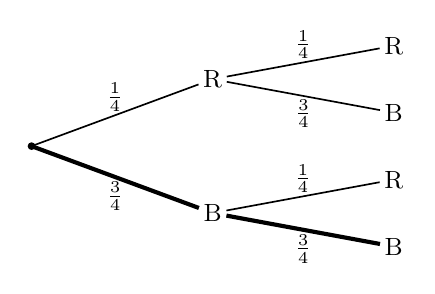
\begin{tikzpicture}[ak/.style={font=\small,inner sep=1.5pt,fill=white},wk/.style={font=\footnotesize,inner sep=1pt}]\fill (0,0) circle (1.4pt);\coordinate (s) at (0,0);\node[ak] (n0) at (2.30,0.850) {R};\node[ak] (n1) at (2.30,-0.850) {B};\node[ak] (n00) at (4.60,1.275) {R};\node[ak] (n01) at (4.60,0.425) {B};\node[ak] (n10) at (4.60,-0.425) {R};\node[ak] (n11) at (4.60,-1.275) {B};\draw[line width=0.6pt] (s) -- (n0) node[wk,above,pos=0.5] {$\frac{1}{4}$};\draw[line width=1.5pt] (s) -- (n1) node[wk,below,pos=0.5] {$\frac{3}{4}$};\draw[line width=0.6pt] (n0) -- (n00) node[wk,above,pos=0.5] {$\frac{1}{4}$};\draw[line width=0.6pt] (n0) -- (n01) node[wk,below,pos=0.5] {$\frac{3}{4}$};\draw[line width=0.6pt] (n1) -- (n10) node[wk,above,pos=0.5] {$\frac{1}{4}$};\draw[line width=1.5pt] (n1) -- (n11) node[wk,below,pos=0.5] {$\frac{3}{4}$};\end{tikzpicture}\end{minipage}\par\medskip
\noindent\textbf{Aufgaben}\hspace{1em}{\small\color{mbgrau}\karohinweis{C}{Rechne unten im Karo.}{Rechne auf einem extra Blatt.} Vergleiche jede Aufgabe gleich mit dem Lösungsheft.}\par\smallskip
\aufgg{\hangindent7mm\hangafter1\nr{1.}Ein Glücksrad hat 5 gleich große Felder, 2 davon sind gold. Es wird zweimal gedreht (G Gold, N nicht Gold). Wie groß ist die Wahrscheinlichkeit für mindestens einmal Gold?}{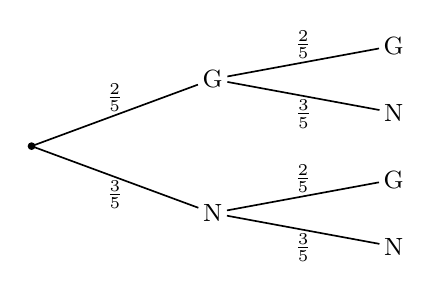
\begin{tikzpicture}[ak/.style={font=\small,inner sep=1.5pt,fill=white},wk/.style={font=\footnotesize,inner sep=1pt}]\fill (0,0) circle (1.4pt);\coordinate (s) at (0,0);\node[ak] (n0) at (2.30,0.850) {G};\node[ak] (n1) at (2.30,-0.850) {N};\node[ak] (n00) at (4.60,1.275) {G};\node[ak] (n01) at (4.60,0.425) {N};\node[ak] (n10) at (4.60,-0.425) {G};\node[ak] (n11) at (4.60,-1.275) {N};\draw[line width=0.6pt] (s) -- (n0) node[wk,above,pos=0.5] {$\frac{2}{5}$};\draw[line width=0.6pt] (s) -- (n1) node[wk,below,pos=0.5] {$\frac{3}{5}$};\draw[line width=0.6pt] (n0) -- (n00) node[wk,above,pos=0.5] {$\frac{2}{5}$};\draw[line width=0.6pt] (n0) -- (n01) node[wk,below,pos=0.5] {$\frac{3}{5}$};\draw[line width=0.6pt] (n1) -- (n10) node[wk,above,pos=0.5] {$\frac{2}{5}$};\draw[line width=0.6pt] (n1) -- (n11) node[wk,below,pos=0.5] {$\frac{3}{5}$};\end{tikzpicture}}{}{}
\medskip
\aufgg{\hangindent7mm\hangafter1\nr{2.}Das Glücksrad im Bild hat 3 gleich große Felder. Es wird zweimal gedreht. Wie groß ist die Wahrscheinlichkeit, dass nicht zweimal Rot kommt? Kreuze an.\par\smallskip\leftskip7mm \kreuz{$\frac{1}{9}$}\ \kreuz{$\frac{4}{9}$}\par\kreuz{$\frac{5}{9}$}\ \kreuz{$\frac{8}{9}$}}{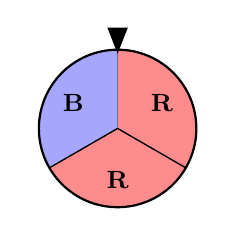
\begin{tikzpicture}[font=\small]\fill[red!45] (0.0,0) -- ++(90.00:1.0) arc (90.00:-30.00:1.0) -- cycle;\draw[line width=0.5pt] (0.0,0) -- ++(90.00:1.0);\node at ([shift=(30.00:0.65)]0.0,0) {\textbf{R}};\fill[red!45] (0.0,0) -- ++(-30.00:1.0) arc (-30.00:-150.00:1.0) -- cycle;\draw[line width=0.5pt] (0.0,0) -- ++(-30.00:1.0);\node at ([shift=(-90.00:0.65)]0.0,0) {\textbf{R}};\fill[blue!35] (0.0,0) -- ++(-150.00:1.0) arc (-150.00:-270.00:1.0) -- cycle;\draw[line width=0.5pt] (0.0,0) -- ++(-150.00:1.0);\node at ([shift=(-210.00:0.65)]0.0,0) {\textbf{B}};\draw[line width=0.8pt] (0.0,0) circle (1.0);\fill (0.0,0.95) -- ++(-0.13,0.33) -- ++(0.26,0) -- cycle;\end{tikzpicture}}{}{}
\medskip
\aufg{\hangindent7mm\hangafter1\nr{3.}Ein roter Würfel trägt die Zahlen 1, 2, 2, 3, 4, 6. Ein blauer Würfel trägt die Zahlen 1, 3, 3, 4, 5, 6. Erst wird der rote, dann der blaue geworfen. Wie groß ist die Wahrscheinlichkeit, dass nicht zweimal eine gerade Zahl fällt?}{}{}
\medskip
\aufg{\hangindent7mm\hangafter1\nr{4.}Bei einem Brettspiel darf Ben zweimal würfeln, um eine 6 zu bekommen. Ben sagt: „Meine Chance ist $\frac{1}{6} + \frac{1}{6} = \frac{1}{3}$.“ Stimmt das? Um wie viel liegt Ben daneben?}{}{{\scriptsize\color{mbgrau}Ziel\hspace{2mm}}}
\medskip
\par\vspace{3mm}\setlength{\kr}{\dimexpr\pagegoal-\pagetotal-10mm\relax}%
\ifdim\kr>12mm\karomerk{k}{C}\noindent{\scriptsize\color{mbgrau}Platz zum Rechnen}\par\nointerlineskip\vspace{1mm}\noindent
\begin{tikzpicture}\clip (0,0) rectangle ({\linewidth-0.5mm},\kr);\draw[black!16,line width=0.3pt,step=5mm] (0,0) grid (\linewidth,\kr);\end{tikzpicture}\fi\par
\clearpage\label{s:D}\noindent\colorbox{black!12}{\makebox[10mm]{\Large\bfseries\strut D}}\hspace{3mm}{\Large\bfseries Drei Stufen}\par\smallskip
\noindent Bei drei Stufen hat jeder Pfad drei Äste, du multiplizierst drei Zahlen. Pfade mit gleich vielen Treffern haben dieselbe Wahrscheinlichkeit.\par\medskip
\noindent\textbf{Formel}\par\nopagebreak\noindent\hspace*{4mm}\begin{minipage}{\dimexpr\linewidth-4mm\relax}$P(\text{Pfad}) = P_1 \cdot P_2 \cdot P_3$ \qquad mindestens zweimal $=$ genau zweimal $+$ dreimal\end{minipage}\par\medskip
\noindent\textbf{Beispiel}\quad Ein Glücksrad hat 4 gleich große Felder: 1 rotes (R) und 3 blaue (B). Es wird dreimal gedreht. Wie groß ist die Wahrscheinlichkeit für genau zweimal Rot?\par\smallskip
\noindent\begin{minipage}[t]{0.6\linewidth}\vspace{0pt}\par\noindent\hangindent6mm\hangafter1\makebox[6mm][l]{\textbf{1}}Genau zweimal Rot: R – R – B, R – B – R, B – R – R.\par\smallskip\par\noindent\hangindent6mm\hangafter1\makebox[6mm][l]{\textbf{2}}Jeder Pfad hat zweimal $\frac{1}{4}$ und einmal $\frac{3}{4}$: $\frac{1}{4} \cdot \frac{1}{4} \cdot \frac{3}{4} = \frac{3}{64}$.\par\smallskip\par\noindent\hangindent6mm\hangafter1\makebox[6mm][l]{\textbf{3}}Drei Pfade addieren: $3 \cdot \frac{3}{64} = \frac{9}{64}$.\par\smallskip\par\noindent\hangindent6mm\hangafter1\makebox[6mm][l]{\textbf{4}}Die Wahrscheinlichkeit für genau zweimal Rot ist $\frac{9}{64}$.\par\smallskip\par\noindent\hangindent6mm\hangafter1\makebox[6mm][l]{\textbf{5}}Mindestens zweimal Rot: dazu kommt dreimal Rot, $\frac{1}{4} \cdot \frac{1}{4} \cdot \frac{1}{4} = \frac{1}{64}$. Zusammen $\frac{9}{64} + \frac{1}{64} = \frac{10}{64} = \frac{5}{32}$.\par\smallskip\end{minipage}\hfill
\begin{minipage}[t]{0.37\linewidth}\vspace{0pt}\centering 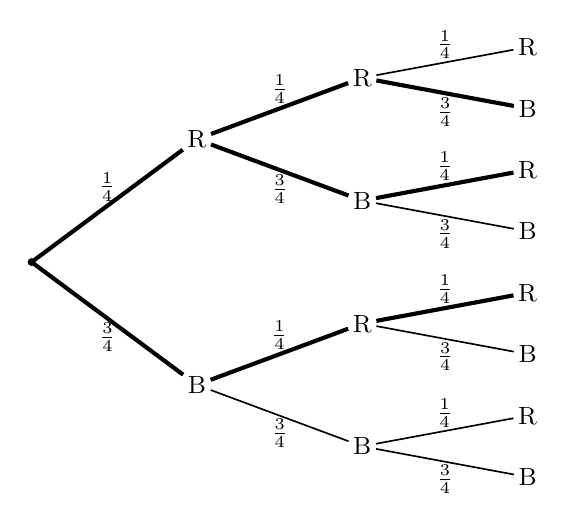
\begin{tikzpicture}[ak/.style={font=\small,inner sep=1.5pt,fill=white},wk/.style={font=\footnotesize,inner sep=1pt}]\fill (0,0) circle (1.4pt);\coordinate (s) at (0,0);\node[ak] (n0) at (2.10,1.560) {R};\node[ak] (n1) at (2.10,-1.560) {B};\node[ak] (n00) at (4.20,2.340) {R};\node[ak] (n01) at (4.20,0.780) {B};\node[ak] (n10) at (4.20,-0.780) {R};\node[ak] (n11) at (4.20,-2.340) {B};\node[ak] (n000) at (6.30,2.730) {R};\node[ak] (n001) at (6.30,1.950) {B};\node[ak] (n010) at (6.30,1.170) {R};\node[ak] (n011) at (6.30,0.390) {B};\node[ak] (n100) at (6.30,-0.390) {R};\node[ak] (n101) at (6.30,-1.170) {B};\node[ak] (n110) at (6.30,-1.950) {R};\node[ak] (n111) at (6.30,-2.730) {B};\draw[line width=1.5pt] (s) -- (n0) node[wk,above,pos=0.5] {$\frac{1}{4}$};\draw[line width=1.5pt] (s) -- (n1) node[wk,below,pos=0.5] {$\frac{3}{4}$};\draw[line width=1.5pt] (n0) -- (n00) node[wk,above,pos=0.5] {$\frac{1}{4}$};\draw[line width=1.5pt] (n0) -- (n01) node[wk,below,pos=0.5] {$\frac{3}{4}$};\draw[line width=1.5pt] (n1) -- (n10) node[wk,above,pos=0.5] {$\frac{1}{4}$};\draw[line width=0.6pt] (n1) -- (n11) node[wk,below,pos=0.5] {$\frac{3}{4}$};\draw[line width=0.6pt] (n00) -- (n000) node[wk,above,pos=0.5] {$\frac{1}{4}$};\draw[line width=1.5pt] (n00) -- (n001) node[wk,below,pos=0.5] {$\frac{3}{4}$};\draw[line width=1.5pt] (n01) -- (n010) node[wk,above,pos=0.5] {$\frac{1}{4}$};\draw[line width=0.6pt] (n01) -- (n011) node[wk,below,pos=0.5] {$\frac{3}{4}$};\draw[line width=1.5pt] (n10) -- (n100) node[wk,above,pos=0.5] {$\frac{1}{4}$};\draw[line width=0.6pt] (n10) -- (n101) node[wk,below,pos=0.5] {$\frac{3}{4}$};\draw[line width=0.6pt] (n11) -- (n110) node[wk,above,pos=0.5] {$\frac{1}{4}$};\draw[line width=0.6pt] (n11) -- (n111) node[wk,below,pos=0.5] {$\frac{3}{4}$};\end{tikzpicture}\end{minipage}\par\medskip
\noindent\textbf{Aufgaben}\hspace{1em}{\small\color{mbgrau}\karohinweis{D}{Rechne unten im Karo.}{Rechne auf einem extra Blatt.} Vergleiche jede Aufgabe gleich mit dem Lösungsheft.}\par\smallskip
\aufg{\hangindent7mm\hangafter1\nr{1.}Ein Glücksrad hat 4 gleich große Felder, eins davon mit Stern. Es wird dreimal gedreht. Wie groß ist die Wahrscheinlichkeit für dreimal Stern?}{}{}
\medskip
\aufgg{\hangindent7mm\hangafter1\nr{2.}Ein Würfel wird dreimal geworfen (6: eine Sechs, k: keine Sechs). Trage im Baum alle Wahrscheinlichkeiten ein. Wie groß ist die Wahrscheinlichkeit, dass keine 6 fällt?}{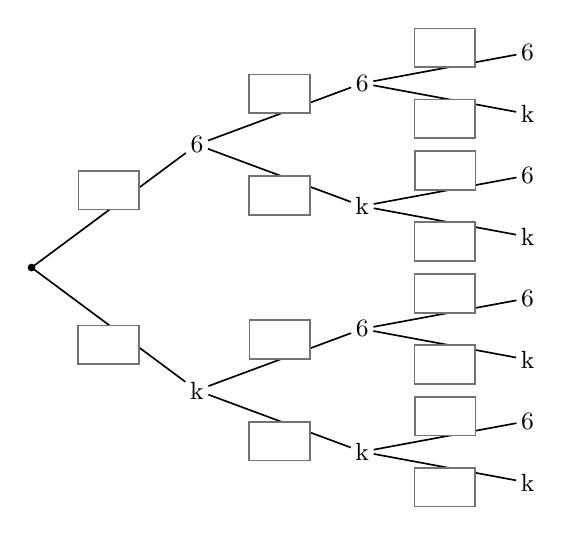
\begin{tikzpicture}[ak/.style={font=\small,inner sep=1.5pt,fill=white},wk/.style={font=\footnotesize,inner sep=1pt}]\fill (0,0) circle (1.4pt);\coordinate (s) at (0,0);\node[ak] (n0) at (2.10,1.560) {6};\node[ak] (n1) at (2.10,-1.560) {k};\node[ak] (n00) at (4.20,2.340) {6};\node[ak] (n01) at (4.20,0.780) {k};\node[ak] (n10) at (4.20,-0.780) {6};\node[ak] (n11) at (4.20,-2.340) {k};\node[ak] (n000) at (6.30,2.730) {6};\node[ak] (n001) at (6.30,1.950) {k};\node[ak] (n010) at (6.30,1.170) {6};\node[ak] (n011) at (6.30,0.390) {k};\node[ak] (n100) at (6.30,-0.390) {6};\node[ak] (n101) at (6.30,-1.170) {k};\node[ak] (n110) at (6.30,-1.950) {6};\node[ak] (n111) at (6.30,-2.730) {k};\draw[line width=0.6pt] (s) -- (n0) node[wk,above,draw=black!55,fill=white,pos=0.5] {\rule{0pt}{4.2mm}\rule{7mm}{0pt}};\draw[line width=0.6pt] (s) -- (n1) node[wk,below,draw=black!55,fill=white,pos=0.5] {\rule{0pt}{4.2mm}\rule{7mm}{0pt}};\draw[line width=0.6pt] (n0) -- (n00) node[wk,above,draw=black!55,fill=white,pos=0.5] {\rule{0pt}{4.2mm}\rule{7mm}{0pt}};\draw[line width=0.6pt] (n0) -- (n01) node[wk,below,draw=black!55,fill=white,pos=0.5] {\rule{0pt}{4.2mm}\rule{7mm}{0pt}};\draw[line width=0.6pt] (n1) -- (n10) node[wk,above,draw=black!55,fill=white,pos=0.5] {\rule{0pt}{4.2mm}\rule{7mm}{0pt}};\draw[line width=0.6pt] (n1) -- (n11) node[wk,below,draw=black!55,fill=white,pos=0.5] {\rule{0pt}{4.2mm}\rule{7mm}{0pt}};\draw[line width=0.6pt] (n00) -- (n000) node[wk,above,draw=black!55,fill=white,pos=0.5] {\rule{0pt}{4.2mm}\rule{7mm}{0pt}};\draw[line width=0.6pt] (n00) -- (n001) node[wk,below,draw=black!55,fill=white,pos=0.5] {\rule{0pt}{4.2mm}\rule{7mm}{0pt}};\draw[line width=0.6pt] (n01) -- (n010) node[wk,above,draw=black!55,fill=white,pos=0.5] {\rule{0pt}{4.2mm}\rule{7mm}{0pt}};\draw[line width=0.6pt] (n01) -- (n011) node[wk,below,draw=black!55,fill=white,pos=0.5] {\rule{0pt}{4.2mm}\rule{7mm}{0pt}};\draw[line width=0.6pt] (n10) -- (n100) node[wk,above,draw=black!55,fill=white,pos=0.5] {\rule{0pt}{4.2mm}\rule{7mm}{0pt}};\draw[line width=0.6pt] (n10) -- (n101) node[wk,below,draw=black!55,fill=white,pos=0.5] {\rule{0pt}{4.2mm}\rule{7mm}{0pt}};\draw[line width=0.6pt] (n11) -- (n110) node[wk,above,draw=black!55,fill=white,pos=0.5] {\rule{0pt}{4.2mm}\rule{7mm}{0pt}};\draw[line width=0.6pt] (n11) -- (n111) node[wk,below,draw=black!55,fill=white,pos=0.5] {\rule{0pt}{4.2mm}\rule{7mm}{0pt}};\end{tikzpicture}}{}{}
\medskip
\aufg{\hangindent7mm\hangafter1\nr{3.}Emma trifft beim Elfmeter mit der Wahrscheinlichkeit $0{,}8$. Sie schießt dreimal. Wie groß ist die Wahrscheinlichkeit für genau zwei Treffer?}{}{}
\medskip
\aufgg{\hangindent7mm\hangafter1\nr{4.}Am Stand gibt es zwei Spiele mit dem Glücksrad im Bild. Spiel A: einmal drehen, du gewinnst bei Stern. Spiel B: dreimal drehen, du gewinnst bei mindestens zwei Sternen. Bei welchem Spiel ist die Gewinnchance größer?}{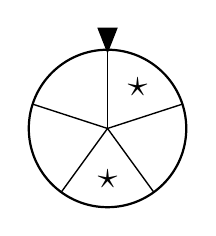
\begin{tikzpicture}[font=\small]\draw[line width=0.5pt] (0.0,0) -- ++(90.00:1.0);\node at ([shift=(54.00:0.65)]0.0,0) {\textbf{\Large$\star$}};\draw[line width=0.5pt] (0.0,0) -- ++(18.00:1.0);\draw[line width=0.5pt] (0.0,0) -- ++(-54.00:1.0);\node at ([shift=(-90.00:0.65)]0.0,0) {\textbf{\Large$\star$}};\draw[line width=0.5pt] (0.0,0) -- ++(-126.00:1.0);\draw[line width=0.5pt] (0.0,0) -- ++(-198.00:1.0);\draw[line width=0.8pt] (0.0,0) circle (1.0);\fill (0.0,0.95) -- ++(-0.13,0.33) -- ++(0.26,0) -- cycle;\end{tikzpicture}}{}{{\scriptsize\color{mbgrau}Ziel\hspace{2mm}}}
\medskip
\par\vspace{3mm}\setlength{\kr}{\dimexpr\pagegoal-\pagetotal-10mm\relax}%
\ifdim\kr>12mm\karomerk{k}{D}\noindent{\scriptsize\color{mbgrau}Platz zum Rechnen}\par\nointerlineskip\vspace{1mm}\noindent
\begin{tikzpicture}\clip (0,0) rectangle ({\linewidth-0.5mm},\kr);\draw[black!16,line width=0.3pt,step=5mm] (0,0) grid (\linewidth,\kr);\end{tikzpicture}\fi\par
\clearpage\label{s:T}\noindent\colorbox{black!12}{\makebox[10mm]{\Large\bfseries\strut T}}\hspace{3mm}{\Large\bfseries Probetest}\par\smallskip
\noindent Gemischt wie in der Prüfung, ohne Beispiel. Taschenrechner erlaubt. Etwa 20 Minuten.\par\medskip
\noindent\textbf{Aufgaben}\hspace{1em}{\small\color{mbgrau}\karohinweis{T}{Rechne unten im Karo.}{Rechne auf einem extra Blatt.} Vergleiche jede Aufgabe gleich mit dem Lösungsheft.}\par\smallskip
\aufgg{\hangindent7mm\hangafter1\nr{1.}Ein grüner Würfel trägt die Zahlen 1, 1, 2, 3, 4, 5. Ein gelber Würfel trägt die Zahlen 2, 2, 4, 5, 6, 6. Erst wird der grüne, dann der gelbe geworfen. Man achtet nur darauf, ob die Zahl gerade (g) oder ungerade (u) ist. Ergänze den Baum. Wie groß ist die Wahrscheinlichkeit, dass beide Zahlen ungerade sind?}{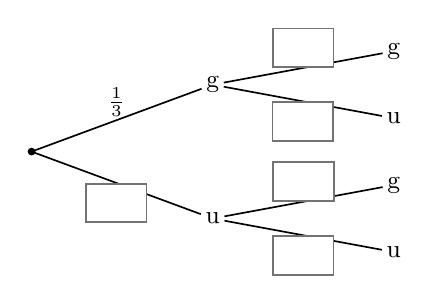
\begin{tikzpicture}[ak/.style={font=\small,inner sep=1.5pt,fill=white},wk/.style={font=\footnotesize,inner sep=1pt}]\fill (0,0) circle (1.4pt);\coordinate (s) at (0,0);\node[ak] (n0) at (2.30,0.850) {g};\node[ak] (n1) at (2.30,-0.850) {u};\node[ak] (n00) at (4.60,1.275) {g};\node[ak] (n01) at (4.60,0.425) {u};\node[ak] (n10) at (4.60,-0.425) {g};\node[ak] (n11) at (4.60,-1.275) {u};\draw[line width=0.6pt] (s) -- (n0) node[wk,above,pos=0.5] {$\frac{1}{3}$};\draw[line width=0.6pt] (s) -- (n1) node[wk,below,draw=black!55,fill=white,pos=0.5] {\rule{0pt}{4.2mm}\rule{7mm}{0pt}};\draw[line width=0.6pt] (n0) -- (n00) node[wk,above,draw=black!55,fill=white,pos=0.5] {\rule{0pt}{4.2mm}\rule{7mm}{0pt}};\draw[line width=0.6pt] (n0) -- (n01) node[wk,below,draw=black!55,fill=white,pos=0.5] {\rule{0pt}{4.2mm}\rule{7mm}{0pt}};\draw[line width=0.6pt] (n1) -- (n10) node[wk,above,draw=black!55,fill=white,pos=0.5] {\rule{0pt}{4.2mm}\rule{7mm}{0pt}};\draw[line width=0.6pt] (n1) -- (n11) node[wk,below,draw=black!55,fill=white,pos=0.5] {\rule{0pt}{4.2mm}\rule{7mm}{0pt}};\end{tikzpicture}}{}{}
\medskip
\aufg{\hangindent7mm\hangafter1\nr{2.}Im Beutel 1 liegen 2 rote und 3 weiße Kugeln, im Beutel 2 eine rote und eine weiße. Aus jedem Beutel wird eine Kugel gezogen. Wie groß ist die Wahrscheinlichkeit für zwei verschiedene Farben? Kreuze an.\par\smallskip\leftskip7mm \kreuz{$\frac{1}{5}$}\ \kreuz{$\frac{3}{10}$}\par\kreuz{$\frac{1}{2}$}\ \kreuz{$\frac{3}{5}$}}{}{}
\medskip
\aufg{\hangindent7mm\hangafter1\nr{3.}Ein Glücksrad hat 8 gleich große Felder, 3 davon sind grün. Es wird zweimal gedreht. Wie groß ist die Wahrscheinlichkeit, mindestens einmal Grün zu drehen? Gib sie auch in Prozent an.}{}{}
\medskip
\aufgg{\hangindent7mm\hangafter1\nr{4.}Ein Glücksrad hat 5 gleich große Felder, eins davon ist gold. Lukas dreht dreimal (G Gold, N nicht Gold). Er gewinnt, wenn mindestens zweimal Gold kommt. Beschrifte alle Äste des Baums. Berechne seine Gewinnwahrscheinlichkeit.}{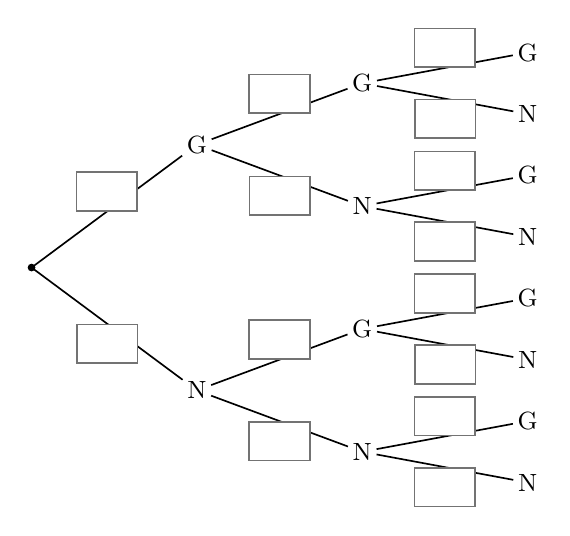
\begin{tikzpicture}[ak/.style={font=\small,inner sep=1.5pt,fill=white},wk/.style={font=\footnotesize,inner sep=1pt}]\fill (0,0) circle (1.4pt);\coordinate (s) at (0,0);\node[ak] (n0) at (2.10,1.560) {G};\node[ak] (n1) at (2.10,-1.560) {N};\node[ak] (n00) at (4.20,2.340) {G};\node[ak] (n01) at (4.20,0.780) {N};\node[ak] (n10) at (4.20,-0.780) {G};\node[ak] (n11) at (4.20,-2.340) {N};\node[ak] (n000) at (6.30,2.730) {G};\node[ak] (n001) at (6.30,1.950) {N};\node[ak] (n010) at (6.30,1.170) {G};\node[ak] (n011) at (6.30,0.390) {N};\node[ak] (n100) at (6.30,-0.390) {G};\node[ak] (n101) at (6.30,-1.170) {N};\node[ak] (n110) at (6.30,-1.950) {G};\node[ak] (n111) at (6.30,-2.730) {N};\draw[line width=0.6pt] (s) -- (n0) node[wk,above,draw=black!55,fill=white,pos=0.5] {\rule{0pt}{4.2mm}\rule{7mm}{0pt}};\draw[line width=0.6pt] (s) -- (n1) node[wk,below,draw=black!55,fill=white,pos=0.5] {\rule{0pt}{4.2mm}\rule{7mm}{0pt}};\draw[line width=0.6pt] (n0) -- (n00) node[wk,above,draw=black!55,fill=white,pos=0.5] {\rule{0pt}{4.2mm}\rule{7mm}{0pt}};\draw[line width=0.6pt] (n0) -- (n01) node[wk,below,draw=black!55,fill=white,pos=0.5] {\rule{0pt}{4.2mm}\rule{7mm}{0pt}};\draw[line width=0.6pt] (n1) -- (n10) node[wk,above,draw=black!55,fill=white,pos=0.5] {\rule{0pt}{4.2mm}\rule{7mm}{0pt}};\draw[line width=0.6pt] (n1) -- (n11) node[wk,below,draw=black!55,fill=white,pos=0.5] {\rule{0pt}{4.2mm}\rule{7mm}{0pt}};\draw[line width=0.6pt] (n00) -- (n000) node[wk,above,draw=black!55,fill=white,pos=0.5] {\rule{0pt}{4.2mm}\rule{7mm}{0pt}};\draw[line width=0.6pt] (n00) -- (n001) node[wk,below,draw=black!55,fill=white,pos=0.5] {\rule{0pt}{4.2mm}\rule{7mm}{0pt}};\draw[line width=0.6pt] (n01) -- (n010) node[wk,above,draw=black!55,fill=white,pos=0.5] {\rule{0pt}{4.2mm}\rule{7mm}{0pt}};\draw[line width=0.6pt] (n01) -- (n011) node[wk,below,draw=black!55,fill=white,pos=0.5] {\rule{0pt}{4.2mm}\rule{7mm}{0pt}};\draw[line width=0.6pt] (n10) -- (n100) node[wk,above,draw=black!55,fill=white,pos=0.5] {\rule{0pt}{4.2mm}\rule{7mm}{0pt}};\draw[line width=0.6pt] (n10) -- (n101) node[wk,below,draw=black!55,fill=white,pos=0.5] {\rule{0pt}{4.2mm}\rule{7mm}{0pt}};\draw[line width=0.6pt] (n11) -- (n110) node[wk,above,draw=black!55,fill=white,pos=0.5] {\rule{0pt}{4.2mm}\rule{7mm}{0pt}};\draw[line width=0.6pt] (n11) -- (n111) node[wk,below,draw=black!55,fill=white,pos=0.5] {\rule{0pt}{4.2mm}\rule{7mm}{0pt}};\end{tikzpicture}}{}{}
\medskip
\aufg{\hangindent7mm\hangafter1\nr{5.}In einen Beutel kommen 10 Kugeln, rote und weiße. Es wird zweimal mit Zurücklegen gezogen. Zweimal Rot soll die Wahrscheinlichkeit $36\,\%$ haben. Wie viele rote Kugeln müssen in den Beutel? Zeige es mit einer Rechnung.}{}{{\scriptsize\color{mbgrau}Ziel\hspace{2mm}}}
\medskip
\par\vspace{3mm}\setlength{\kr}{\dimexpr\pagegoal-\pagetotal-10mm\relax}%
\ifdim\kr>12mm\karomerk{k}{T}\noindent{\scriptsize\color{mbgrau}Platz zum Rechnen}\par\nointerlineskip\vspace{1mm}\noindent
\begin{tikzpicture}\clip (0,0) rectangle ({\linewidth-0.5mm},\kr);\draw[black!16,line width=0.3pt,step=5mm] (0,0) grid (\linewidth,\kr);\end{tikzpicture}\fi\par
\end{document}
